% Asset ID: FA22CentralLimitTheoremTikZ-002
% Used placeholder: [VISUAL PLACEHOLDER: FA22CentralLimitTheoremTikZ-002 | Source: Teacher transcript minimum sample-size method | Insert from tikz/FA22CentralLimitTheoremTikZ-002.tex | Purpose: Show why a strict tail-probability inequality becomes an inequality for n.]
\documentclass[tikz,border=8pt]{standalone}
\usepackage{amsmath}
\usetikzlibrary{arrows.meta}
\definecolor{Canvas}{HTML}{FAF9F6}\definecolor{Gold}{HTML}{C5A059}\definecolor{Rose}{HTML}{FBEFEF}\definecolor{Ink}{HTML}{2C2C2E}
\begin{document}
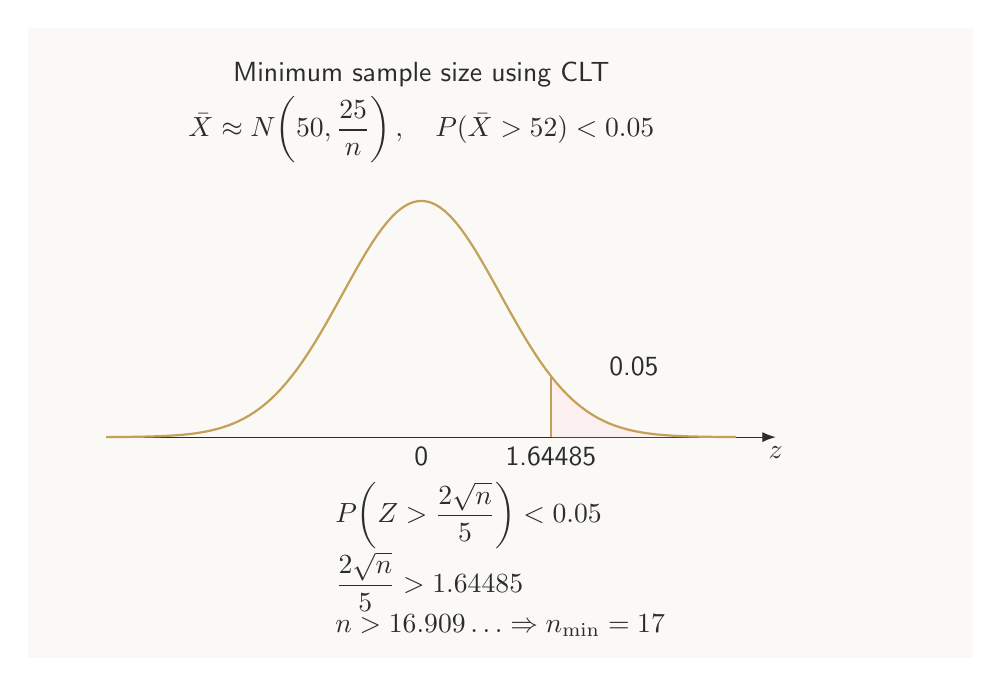
\begin{tikzpicture}[>=Latex,every node/.style={font=\sffamily,text=Ink}]
\fill[Canvas] (-5,-2.8) rectangle (7,5.2);
\node at (0,4.6){Minimum sample size using CLT};
\node at (0,3.9){$\bar X\approx N\!\left(50,\dfrac{25}{n}\right),\quad P(\bar X>52)<0.05$};
\draw[Ink,->] (-4,0)--(4.5,0) node[below]{$z$};
\def\z{1.64485}
\path[fill=Rose] (\z,0)--plot[domain=\z:4,samples=80](\x,{3*exp(-.5*\x*\x)})--(4,0)--cycle;
\draw[Gold,thick,samples=120,domain=-4:4] plot(\x,{3*exp(-.5*\x*\x)});
\draw[Gold,thick] (\z,0)--(\z,{3*exp(-.5*\z*\z)});
\node[below] at (0,0){0};\node[below] at (\z,0){1.64485};\node at (2.7,.9){0.05};
\node[align=left] at (1,-1.55){$P\!\left(Z>\dfrac{2\sqrt n}{5}\right)<0.05$\\$\dfrac{2\sqrt n}{5}>1.64485$\\$n>16.909\ldots\Rightarrow n_{\min}=17$};
\end{tikzpicture}
\end{document}
